\documentclass[a4paper]{article}
\usepackage[utf8]{inputenc}
\usepackage[T1]{fontenc}
\usepackage{graphics}
\usepackage{libertine}
\usepackage{tango}
%\usepackage[colorlinks=true]{hyperref}

\hypersetup{urlcolor=DarkChocolate}

\title{TP Git}
%\author{\scalebox{0.35}{ \includegraphics{logo_azae}}}
\author{Thomas Clavier}
\date{}

\setlength{\parindent}{0pt}
\newcounter{question}
\setcounter{question}{1}
\newcommand{\q}{
  \textcolor{DarkOrange}{\textbf{Question \thequestion : }}
  \addtocounter{question}{1}
  \newline
}

\begin{document}

\maketitle

\section*{Préparation}
Avant toute chose aller sur le serveur gitlab de l'IUT : \url{https://git.iut-info.univ-lille1.fr} et se connecter avec le login des salles de TP.

\section*{Présentation}

\subsection*{Des objets}
Un dépôt Git peut être vu comme une collection d’objets liés entre eux. 
Chaque objet est identifié par une chaîne de 40 caractères hexadécimaux
correspondant à la somme de contrôle de son contenu. 
Il y a 3 types d'objets : 
\begin{itemize}
\item blob : les données
\item tree : les arborescences
\item commit : une version du répertoire de travail
\end{itemize}
Un objet de type <<arborescence>> peut contenir des objets <<données>> et <<arborescence>>.
Le répertoire de travail est lui-même un objet de type <<arborescences>>. 

L'historique d'un dépôt Git c'est l'ensemble des versions du répertoire de travail. Pour identifier une version, Git s'appuie sur un objet de type <<commit>>. 
L'objet de type <<commit>> associe de nombreuses informations comme l'auteur, un message, une version de l'objet répertoire de travail mais aussi les <<commits> parents.

%TODO 3 schémas : graph de versions (branches) graphs de commits et tree + blob

\subsection*{Les espaces}
Git utilise 3 espaces différents pour manipuler toutes ces données.
\begin{itemize}
\item le répertoire de travail
\item l'index
\item l'historique
\end{itemize}

Le répertoire de travail présente dans un dossier de la machine, l'ensemble des fichiers du dépôt. C'est le point d'entrée de l'utilisateur.

L'index contient les données en préparation pour le commit

La tête (HEAD) de l'historique contient le dernier commit.

\scalebox{0.7}{ 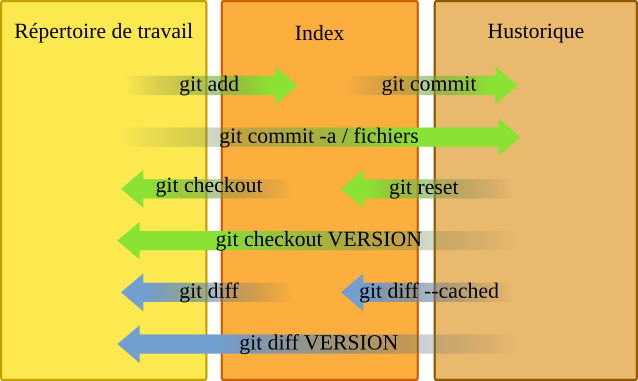
\includegraphics{espaces}}

\subsection*{configuration}

Configuration de git :

\begin{verbatim}
git config --global user.email jean.dupont@example.com 
git config --global user.name 'Jean Dupont'
\end{verbatim}

\section*{L'espace de travail}

À partir de là nous allons construire un annuaire en ligne de tous les élèves de la promotion. 

\subsection*{Initialisation}
Création d'un dépôt local
\begin{verbatim}
mkdir /tmp/annuaire
cd /tmp/annuaire
git init .
\end{verbatim}

\subsection*{Historique de version}
Création d'un premier fichier à votre nom, il contiendra votre CV au format Markdown (\url{http://daringfireball.net/projects/markdown/syntax}).
Pour ce premier commit nous allons le créer avec juste votre nom dedans :
\begin{verbatim}
echo "#Prénom Nom" > nom-prenom.mkd
\end{verbatim}

L'ajouter dans l'index comme fichier à suivre
\begin{verbatim}
git add nom-prenom.mkd
\end{verbatim}

Validez l'index pour créer un commit
\begin{verbatim}
git commit -m "première version du cv de Nom Prénom"
\end{verbatim}

\q Observez l'historique des changements, quelles sont les informations disponibles ? À quoi correspond chaque champ ?
\begin{verbatim}
git log
\end{verbatim}

\q Pour avoir de l'aide sur git, il est possible de lancer "man git". Pour
avoir de l'aide sur la commande "git log" il est possible de lancer "man
git-log".

Comment avoir l'affichage suivant : 
\begin{verbatim}
commit 062f166cbbd729a90a30a31578f10953d7a05dc5
Author: Nom Prénom <prenom.nom@example.com>
Date:   Sun Mar 1 11:49:45 2034 +0100

    première version du cv de Nom Prénom

 nom-prenom.mkd | 5 ++++
 1 file changed, 1 insertion(+)
\end{verbatim}

\q Que représentent les "+"  ?

Ajoutez quelques informations dans votre CV.
\begin{verbatim}
gedit nom-prenom.mkd
git commit -m "Une version plus à jour du CV de mon CV" -a
\end{verbatim}

\q Que font les commandes suivantes :
\begin{verbatim}
echo "Une nouvelle ligne" >> nom-prenom.mkd
git blame nom-prenom.mkd
git status
git diff
git commit -m "Commit uniquement pédagogique" -a
\end{verbatim}

\q Comment obtenir le diff entre les 2 derniers commits ?

Créez le CV de Satoshi Tajiri
\begin{verbatim}
gedit satoshi-tajiri.mkd
git add satoshi-tajiri.mkd
git commit -m "Ajout du Cv de Satoshi Tajiri"
\end{verbatim}

Nous construisons l'annuaire de la promo ... 
\begin{verbatim}
git rm satoshi-tajiri.mkd
git commit -m "suppession du CV de Satoshi Tajiri"
\end{verbatim}

\q Que voit-on dans l'historique (git log) ?

Tous les CV sont au format Markdown mais nous allons publier du html.
Nous allons déplacer les CV dans un sous répertoire cv pour bien séparer le code html des cv.

\begin{verbatim}
mkdir cv
git mv nom-prenom.mkd cv/nom-prenom.mkd
git commit -m "Création du répertoire cv"
\end{verbatim}

\q Quel aurait été le résultat si nous avions remplacé le git mv par les 3 commandes suivantes :
\begin{verbatim}
mv nom-prenom.mkd cv/nom-prenom.mkd
git add cv/nom-prenom.mkd
git rm nom-prenom.mkd
\end{verbatim}

\section*{Partager}

\subsection*{Via un dépôt partagé}

Ajouter votre clé ssh sur le serveur gitlab : 
\url{https://git.iut-info.univ-lille1.fr/profile/keys/new}


Dans le champ "Key" coller le contenu du fichier <<\textasciitilde/.ssh/id\_rsa.pub>>.
Si ce fichier n'existe pas, le créer avec la commande ssh-keygen.

Dans le champ Title donner un nom à votre clé, par exemple <<tp iut>>.

Indiquons à Git que nous souhaitons échanger des données avec le dépôt distant suivant : git@git.iut-info.univ-lille1.fr:thomas.clavier/2014tpgits2.git
Nous appelons ce dépôt <<origin>>.

\begin{verbatim}
git remote add origin \
git@git.iut-info.univ-lille1.fr:thomas.clavier/2014tpgits2.git
\end{verbatim}

Envoyons l'ensemble des modifications de la branche courante (master) vers le dépôt <<origin>>

\begin{verbatim}
git push origin master
\end{verbatim}

\q Que se passe-t-il ?

\q Pour récupérer le travail fait par le reste du groupe avant d'envoyer ses propres modifications il suffit de lancer : 

\begin{verbatim}
git pull 
\end{verbatim}

Avant de renvoyer le tout sur le serveur :
\begin{verbatim}
git push origin master
\end{verbatim}

Expliquez le résultat de la commande suivante : 
\begin{verbatim}
git log --oneline --graph --decorate
\end{verbatim}

Si l'on souhaite obtenir une copie de travail d'un dépôt distant existant il est possible d'utiliser la commande :
\begin{verbatim}
git clone url
\end{verbatim}

\q Quelles sont les formes d'URL possibles ?

Lançons la génération des pages html : 
\begin{verbatim}
make html
\end{verbatim}

\q Que donne la commande suivante ? Pourquoi ? 
\begin{verbatim}
git status
\end{verbatim}

\q Est-il normale d'enregistrer du code généré ? 

Pour ignorer tout le répertoire de génération modifions le fichier .gitignore
\begin{verbatim}
gedit .gitignore
\end{verbatim}

Lancez la commande suivante :
\begin{verbatim}
make pok
\end{verbatim}
\q Expliquez ce qui s'est passé. Vous pouvez utiliser la commande "git status" pour vous aider.

\q Que fait la commande suivante ?
\begin{verbatim}
git clean -f
\end{verbatim}

Modifiez le fichier changelog pour indiquer que la nouvelle version de l'annuaire comporte votre nom
\begin{verbatim}
gedit changelog
\end{verbatim}

\q Enregistrez et partagez vos modifications, que se passe-t-il ? 

\q À quoi correspondent les lignes suivantes : 
\begin{verbatim}
<<<<<<< HEAD
DD MM YYYY : Monsieur Patate <monsieur@patate.org>
- Monsieur Patate est dans l'annuaire
=======
DD MM YYYY : Madame Patate <madame@patate.org>
- Madame Patate est dans l'annuaire
>>>>>>> branch-a
\end{verbatim}

\q Comment résoudre ce problème ?

\subsection* {Par mail}

\begin{verbatim}
git format-patch
git send-email
git archive
\end{verbatim}

\section*{Gérer le code}

Pour identifier un commit avec un nom facile à retenir, il est possible de poser un tag. C'est par exemple utilisé pour marquer une version donnée.

\begin{verbatim}
git tag 1.0.0
\end{verbatim}

\subsection*{Des branches}

Pour gérer plusieurs versions de l'ensemble du code en parallèle, Git propose de faire des <<branches>>.

\q
\begin{itemize}
  \item Ajoutez une branche "nom-prenom-merge", 
  \item dans cette branche modifiez votre CV (en fin de fichier), puis commitez (faire au moins 2 modifications et 2 commits). 
  \item Revenez sur la branche master, 
  \item faites 2 modifications en début de fichiers (avec 2 commits) 
  \item puis fusionnez la branche "nom-prenom" avec master.
\end{itemize}

\begin{verbatim}
git merge nom-prenom-merge
\end{verbatim}

Observez le résultat dans l'arbre des versions. 
\begin{verbatim}
git log --graph --oneline --all
\end{verbatim}

Expliquer ce qui c'est passé.

\q
\begin{itemize}
  \item Ajoutez une branche "nom-prenom-rebase", 
  \item dans cette branche modifiez votre CV, puis commitez (faire au moins 2 modifications et 2 commits). 
  \item Revenez sur la branche master, 
  \item et faites à nouveau 2 modifications en début de fichier (avec 2 commits) 
  \item puis <<rebasez>>.
\end{itemize}
\begin{verbatim}
git rebase nom-prenom-rebase
\end{verbatim}

Observez le résultat dans l'arbre des versions. 
\begin{verbatim}
git log --graph --oneline --all
\end{verbatim}

Expliquer ce qui c'est passé.

\q Au moment de faire un pull pour rapatrier le travail du reste de l'équipe, il est possible de faire un pull rebase.

\begin{verbatim}
git pull -r
\end{verbatim}
Expliquer ce que fait cette commande.

\section*{Plus loin}

\q Expliquez chacune des commandes suivantes :
\begin{verbatim}
git log --graph --pretty=format:\
'%Cred%h%Creset -%C(yellow)%d%Creset \
%s %C(bold blue)<%an>%Creset%n' --abbrev-commit --all
git stash 
git stash pop
git bisect
git staged
git unstage
git fix 
\end{verbatim}


\end{document}

